%
% Chapter 4
%

\chapter{PHYSICS OBJECTS}
Each of the CMS subdetectors (neglecting the trigger system) technically only record and detect hits and energy deposits. While these hits and energy deposits are almost
always due to passing particles, the detectors themselves and more precisely the readouts, only produce information about the position, value, and multiplicity of
these hits and energy deposits. It is thanks to clever and accurate experimental techniques that we can reconstruct various particles from these hits and energy deposits.
In part because CMS does not detect particles directly, reconstructed particles are referred to as physics \emp{objects} in this context. Using
the term particles implies certainty about the identify of the object, and because there is some uncertainty, however small, inherent in the reconstruction, objects is
more accurate and widely used. The reconstruction technique varies greatly with different objects and the subdetectors used to detect and record their hits and energy
deposits. 

\section{Particle Flow}
The particle flow algorithm is used by CMS to reconstruct physics objects from hits and energy deposits. Particle Flow and CMS are unique in the sense
that nearly all physics analyses performed on data collected by CMS use objects reconstructed with this single algorithm. The primary advantage of this strategy is
uniform and consistent object definitions across nearly all papers published on behalf of CMS. Other collaborations such as ATLAS do not use
the same algorithm collaboration-wide. The purpose of particle flow is to identify all final-state stable particles in an event recorded by CMS, specifically electrons,
mouons, taus, jets and photons. Particle flow optimally combines building-block information (hits and energy clusters) from all subdetectors to reconstruct objects and
determine particle type, position, and momentum. 


\begin{figure}[hbtp]
 \begin{center}
   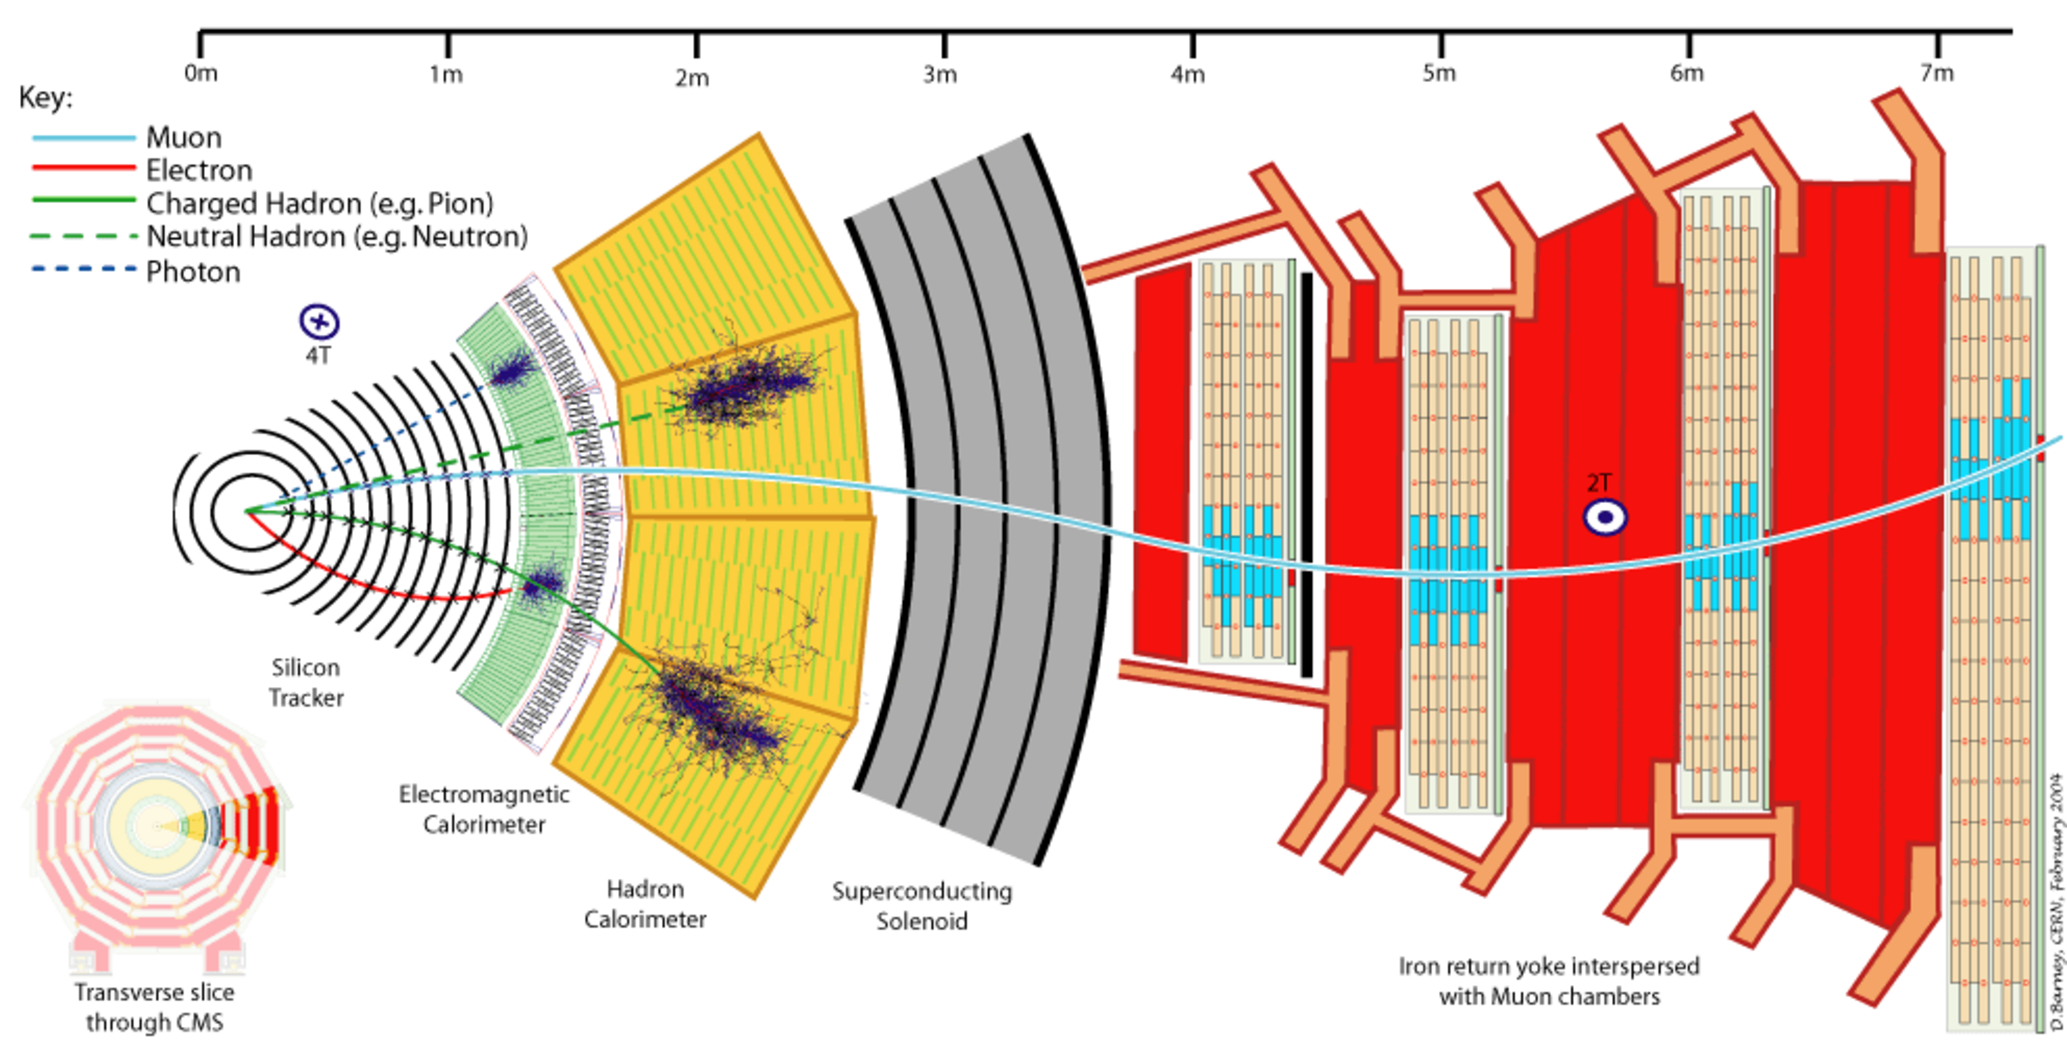
\includegraphics[width=0.8\textwidth]{ch4_figs/cms_particleflow.pdf}
   \caption{An overview of how CMS detects different types of particles. The slice of CMS in in the x-y plane.~\cite{NEED CITATION}.}
   \label{fig:cms_pflow}
 \end{center}
\end{figure}

Object reconstruction begins with grouping collections of hits into tracks, in an iterative process~\cite{CMS-TRK-09-001}. In the first iteration, tracks are
seeded with initial hits and subject to very tight criteria, sacrificing efficiency for a low fake rate. In the following iterations, hits assigned to
tracks in the previous iteration are removed from further consideration, and the criteria for candidate tracks is gradually relaxed with each iteration. In the final iterations,
the constraints on the track seed are relaxed to account for secondary decays from photon conversions and nuclear interactions with the silicon tracker material. This technique
reconstructs tracks with as few as three hits and \pts as small as 150 MeV with a fake rate in the single digits~\cite{CMS-PFT-09-001}. 


\section{Jets}
\section{Leptons}
\section{Taus}
\section{MET}

